\documentclass[aspectratio=43]{beamer}

%%%%%%%%%%%%%%%%%%%%%%%%%%%%%%%%%%%%%%%%%%%%%%%%%%%%%%%%%%%%%%%%%%%%
% über aspectratio kann das Format eingestellt werden. Der Default
% wert ist 43 (4:3, 128mm:96mm). Andere Möglichkeiten sind
% 32 (3:2, 135mm:90mm)
% 54 (5:4, 125mm:100mm)
% 149 (14:9, 14cm:9cm)
% 169 (16:9, 16cm:9cm)
% 1610 (16:10, 16cm:10cm)
% 141 (1.41:1, 148.5mm:105mm, Seitenverhältnis wie bei DIN-A)
%%%%%%%%%%%%%%%%%%%%%%%%%%%%%%%%%%%%%%%%%%%%%%%%%%%%%%%%%%%%%%%%%%%%


\usepackage[T1]{fontenc}
\usepackage[utf8x]{inputenc}
\usepackage[ibycus,ngerman]{babel}
\usepackage{amsfonts,amsmath,amssymb,amsthm}
\usepackage{csquotes}

\usepackage{hyperref}




\usetheme[komms=false]{fbmathematik}

%%%%%%%%%%%%%%%%%%%%%%%%%%%%%%%%%%%%%%%%%%%%%%%%%%%%%%%%%%%
% Schriftfarben:
% tuklblau, tuklrot, warmgrau, kaltgrau;
% abgeschwächte Töne für die obigen Farben und schwarz:
% z.B. tuklblau7 für 70% tuklblau, warmgrau2 für 20%
% warmgrau oder schwarz6 für 60% schwarz,
% jeweils in den Schritten 10%, 20%, 40%, 60%, 70%, 80%;
% violette Schriftfarbe (Felix-Klein) hat den Namen fkz1
% hellviolette FKZ-Variante hat den Namen fkz2;
% KOMMS: kommsblau, kommsgruen, kommsgrau, kommsblaugrau
%%%%%%%%%%%%%%%%%%%%%%%%%%%%%%%%%%%%%%%%%%%%%%%%%%%%%%%%%%%



\title{Projektvorstellung: Immer der Sonn' entgegen}
\author{Dominik Bendle \and Melissa Hasel \and Thomas Hofmann}
\date{\today}
\institute{TU Kaiserslautern}

\begin{document}

\begin{frame}[plain]

\Titel{logo}

\end{frame}

\begin{frame}
    \frametitle{Immer der Sonn' entgegen}
    \begin{itemize}
        \item Gegeben: Beliebiger zugänglicher Punkt auf der Erde.
        \item Gesucht: Pfad und Endpunkt, wenn einen Tag lang immer in Richtung Sonne
            gelaufen/gewandert/\dots{} wird. Dabei werden Hindernisse und Barrieren sowie
            notwendige oder freiwillige Laufpausen berücksichtigt.
    \end{itemize}
\end{frame}

\begin{frame}[plain]
    \frametitle{Arbeitsplanung und Fragestellungen}
    \begin{itemize}
        \item Erstellung einfacher Sonnen-Erd-Modelle für einfache Berechnung der
            Sonnenposition
        \item[] $\rightarrow$ ohne und mit Achsenneigung der Erde
        \item[] $\rightarrow$ zum Ende des Projekts evtl. Vergleich mit echten Daten
        \item Implementierung der \enquote{Sonnenverfolgung} auf einer optimalen/leeren Erde.
        \item[] $\rightarrow$ variable Laufgeschwindigkeit
        \item Entwicklung einer (rudimentären) graphischen Oberfläche zur Darstellung der
            Karte und des Pfades.
        \item Einbezug echter Kartendaten (z.B. OpenStreetMap)
        \item[] $\rightarrow$ zunächst Weg entlang Straßen und Wege
        \item[] $\rightarrow$ sofern Qualität der Karten dies erlaubt: Weg querfeldein
            ohne Straßen-/Wegbindung.
        \item[] $\rightarrow$ Frage: Was tun wenn sich nicht in Richtung der Sonne bewegt
            werden kann?
    \end{itemize}
\end{frame}

\begin{frame}
    \begin{itemize}
        \item Einbezug echter Kartendaten (z.B. OpenStreetMap)
        \item[] $\rightarrow$ zunächst Weg entlang Straßen und Wege
        \item[] $\rightarrow$ sofern Qualität der Karten dies erlaubt: Weg querfeldein
            ohne Straßen-/Wegbindung.
        \item[] $\rightarrow$ Frage: Was tun wenn sich nicht in Richtung der Sonne bewegt
            werden kann?
    \end{itemize}
\end{frame}

\begin{frame}
    \begin{center}
        \begin{figure}[t]
            \centering
            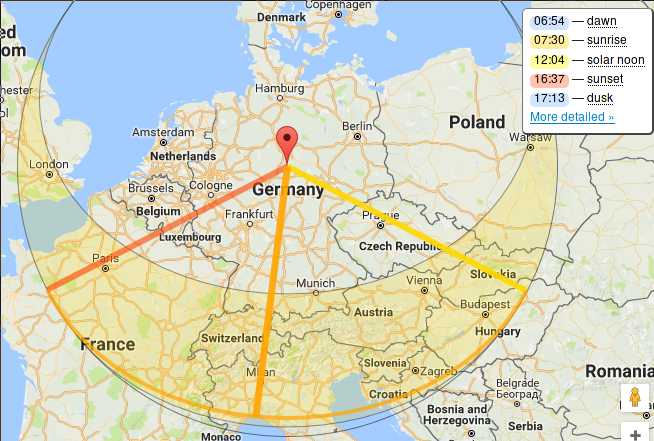
\includegraphics[width=0.7\textwidth]{bilder/suncalc.png}
            \caption{Genaue Bestimmung der Sonne; Screenshot von \url{suncalc.net}}
        \end{figure}
    \end{center}
\end{frame}

\begin{frame}
    \begin{center}
        \begin{figure}[t]
            \centering
            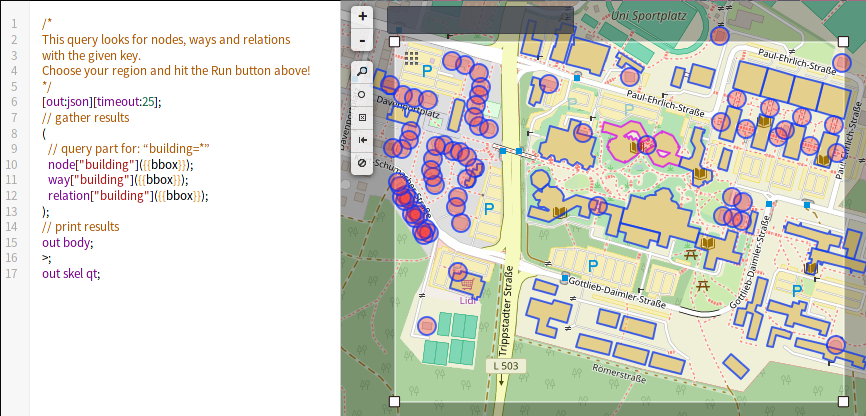
\includegraphics[width=0.99\textwidth]{bilder/overpass.png}
            \caption{OpenStreetMap-Daten für Gebäude und Barrieren zur
            Kollisionsbestimmung oder auch Straßendaten; Screenshot von
            \url{overpass-turbo.eu}}
        \end{figure}
    \end{center}
\end{frame}

\end{document}

